\section{Numerical studies}\label{sec:numerical-study}
\newcommand{\TotalReplications}{54,000}


\subsection{Simulation design and competing methods}\label{subsec:simulation}

The factorial design compares nominal 95\% bands with $n\in\{200,400\}$ subjects, $m\in\{5,20,80\}$ observations per subject, and Gaussian, Laplace, or adjusted chi-square innovations in the functional errors. We refer to these three sampling frequencies as sparse, mild, and dense; these are finite-sample labels. Every configuration uses $R=1{,}000$ independent datasets. We examine a single coefficient in a two-coefficient model, simultaneous coverage of all five coefficients in a five-coefficient model, and the extension to mean functions in Section~\ref{sec:mean-model}.

Observation times are independent Uniform$(0,1)$. Predictors and the single functional error are generated from smooth finite-basis processes. Error innovations have mean zero and variance one: $N(0,1)$, Laplace$(0,1/\sqrt2)$, or $(\chi^2_5-5)/\sqrt{10}$. The latter two examine heavier symmetric tails and positive skewness, respectively. The coefficient functions include linear, oscillating, quadratic, and exponential trends. Section~\ref{app:simulation-design} gives the complete generating mechanism and targets. We use local linear fits with the Epanechnikov kernel, one common bandwidth for the estimate and residuals, and $B=2000$ Gaussian multiplier draws. Both methods in each comparison use the same 201 equally spaced evaluation points in $[0,1]$. In the tables, Coverage is the proportion of datasets in which all targeted coefficients are covered at every evaluation point; Width is the band width averaged over datasets, evaluation points, and targeted coefficients.

For coefficient bands, we compare with \citet{cao_simultaneous_2018}, abbreviated CLZ. Both local linear estimators use the same bandwidth; with equal counts their point estimates agree, while covariance estimation and calibration differ. The CLZ limit theory calibrates a scalar process for a prespecified contrast of the coefficient vector and does not provide joint calibration over multiple coefficient functions. For the five-function target, we therefore construct each marginal band at level $1-0.05/5=0.99$, using Bonferroni correction across the five coefficients for a nominal 95\% joint comparison. Section~\ref{app:comparator-formulas} specifies its kernel variance estimates and finite-observation Gaussian calibration. The CLZ theory concerns sparse longitudinal sampling, so its mild and dense entries assess performance beyond that regime.

For the mean problem, we compare with the B-spline bands of \citet{cai_hu_2025}, which also accommodate varying sampling frequencies. Their cubic-spline fit uses BIC-selected knots and a subject-score covariance estimate. The design, full results, and computational details for this specialization are in Section~\ref{app:numerics}.

\subsection{Coverage and width}

\begin{table}[!tbp]
\centering
\caption{Coverage probability (CP) and average width (AW) of nominal 95\% bands for all five coefficients jointly. Each row uses 1,000 datasets; $m=5,20,80$ denote sparse, mild, and dense sampling.}
\label{tab:joint-new}
\renewcommand{\baselinestretch}{1.2}\small
\begin{tabular}{llrrrrr}
\toprule
& & & \multicolumn{2}{c}{Proposed} & \multicolumn{2}{c}{CLZ (Bonferroni)}\\
Innovations & $n$ & $m$ & CP & AW & CP & AW\\
\midrule
Gaussian & 200 & 5 & 0.822 & 0.703 & 0.458 & 0.566\\
 & 200 & 20 & 0.906 & 0.545 & 0.042 & 0.288\\
 & 200 & 80 & 0.912 & 0.497 & 0.000 & 0.144\\
 & 400 & 5 & 0.910 & 0.556 & 0.581 & 0.458\\
 & 400 & 20 & 0.919 & 0.412 & 0.073 & 0.229\\
 & 400 & 80 & 0.940 & 0.362 & 0.000 & 0.115\\
\midrule
Laplace & 200 & 5 & 0.871 & 0.698 & 0.491 & 0.565\\
 & 200 & 20 & 0.904 & 0.543 & 0.047 & 0.288\\
 & 200 & 80 & 0.914 & 0.492 & 0.000 & 0.143\\
 & 400 & 5 & 0.904 & 0.550 & 0.618 & 0.454\\
 & 400 & 20 & 0.925 & 0.410 & 0.063 & 0.228\\
 & 400 & 80 & 0.929 & 0.361 & 0.001 & 0.115\\
\midrule
Adjusted $\chi^2_5$ & 200 & 5 & 0.847 & 0.698 & 0.484 & 0.563\\
 & 200 & 20 & 0.901 & 0.545 & 0.044 & 0.289\\
 & 200 & 80 & 0.910 & 0.494 & 0.000 & 0.144\\
 & 400 & 5 & 0.885 & 0.553 & 0.580 & 0.457\\
 & 400 & 20 & 0.924 & 0.410 & 0.064 & 0.229\\
 & 400 & 80 & 0.934 & 0.362 & 0.000 & 0.115\\
\bottomrule
\end{tabular}
\end{table}


Table~\ref{tab:joint-new} reports joint coverage and width for every sampling frequency and all three innovation distributions. Table~\ref{tab:single-new} in the supplement gives the single-coefficient comparison.

The proposed single-coefficient CP ranges from 0.908 to 0.948, compared with 0.052 to 0.773 for CLZ. For joint inference the ranges are 0.822--0.940 and 0.000--0.618, respectively. The proposed coverage is closer to 0.95 in all 36 coefficient-model configurations. Comparing $m=5$ with $m=80$ at each fixed target, subject sample size, and error law, both CLZ width and coverage decrease in all twelve comparisons.

For the proposed joint bands, CP at $n=200$ ranges from 0.822 to 0.914. At $n=400$ the corresponding range is 0.885--0.940. These ranges make the remaining finite-sample coverage error explicit. Both Gaussian and non-Gaussian results are reported without selecting configurations by outcome.

For the mean comparison in Table~\ref{tab:mean-new}, proposed CP is 0.919--0.954, while Cai--Hu CP is 0.932--0.958. Cai--Hu bands are narrower in all 18 mean configurations. Coverage and width should be interpreted together under the specified tuning parameters.


For Gaussian joint bands, increasing $m$ from 20 to 80 changes coverage from 0.906 to 0.912 at $n=200$, and from 0.919 to 0.940 at $n=400$. The two coverage differences have Monte Carlo standard errors 0.013 and 0.011, respectively. Average widths decrease from 0.545 to 0.497 and from 0.412 to 0.362. The smoothing bandwidth is unchanged across $m$ at each fixed $n$ under the prespecified rule. Coverage reflects calibration error and smoothing bias as well as variance, so coverage and width need not change in parallel.


\subsection{Multivariate functional means}\label{subsec:highd-mean-simulation}

To examine the multivariate mean procedure in
Corollary~\ref{cor:hdmean}, we consider $n=200,400$ subjects,
$m=5,20,80$ observations per subject, and $p=50,100$ mean functions.
The functional errors combine common
and coordinate-specific innovations from the same three distributions
as above, with cross-coordinate correlation $1/2$.
The procedure uses coordinate-specific residuals and variance estimates,
with a common subject multiplier and one joint bootstrap maximum.
The generating processes satisfy the coordinate moment and covariance
conditions of the corollary. Their envelope grows at most as
$\sqrt{\log(ep)}$ for Gaussian innovations and $\log(ep)$ for the
other two innovation laws. The displayed rate conditions remain
asymptotic requirements; they do not guarantee nominal coverage at
these finite sample sizes.
Each $(n,m,\text{innovation law})$ uses 1,000 independent datasets and
999 subject multiplier draws. The two dimensions are nested coordinate
prefixes of the same datasets and use the same multipliers. All 36
configurations are evaluated under this fixed design.
Coverage requires all coordinates at all 51 equally spaced points on
$[0,1]$, including endpoints. The shared scalar design permits computation
in response blocks while retaining a single joint bootstrap critical value.
Section~\ref{app:highd-mean-simulation} specifies the curves, random streams,
bandwidth, implementation checks, and timing convention.

\begin{table}[!tbp]
\centering
\caption{Joint grid coverage (CP) and average width (AW) for multivariate functional means with $n=200,400$, $m=5,20,80$, and $p=50,100$. All configurations are reported. Each cell uses 1000 datasets and 999 subject multipliers on 51 points spanning $[0,1]$.}
\label{tab:highd-mean}
\small
\setlength{\tabcolsep}{4pt}
\begin{tabular}{rrrrrrrrr}
\toprule
& & & \multicolumn{2}{c}{Gaussian} & \multicolumn{2}{c}{Laplace} & \multicolumn{2}{c}{Adjusted $\chi^2_5$}\\
$n$ & $m$ & $p$ & CP & AW & CP & AW & CP & AW\\
\midrule
200 & 5 & 50 & 0.860 & 0.927 & 0.878 & 0.927 & 0.802 & 0.926\\
200 & 5 & 100 & 0.842 & 0.961 & 0.855 & 0.961 & 0.782 & 0.959\\
\midrule
200 & 20 & 50 & 0.907 & 0.692 & 0.920 & 0.693 & 0.883 & 0.690\\
200 & 20 & 100 & 0.904 & 0.719 & 0.920 & 0.719 & 0.877 & 0.717\\
\midrule
200 & 80 & 50 & 0.911 & 0.605 & 0.929 & 0.603 & 0.913 & 0.604\\
200 & 80 & 100 & 0.915 & 0.630 & 0.927 & 0.628 & 0.903 & 0.629\\
\midrule
400 & 5 & 50 & 0.924 & 0.716 & 0.925 & 0.715 & 0.865 & 0.714\\
400 & 5 & 100 & 0.909 & 0.741 & 0.908 & 0.740 & 0.848 & 0.740\\
\midrule
400 & 20 & 50 & 0.933 & 0.515 & 0.930 & 0.514 & 0.932 & 0.515\\
400 & 20 & 100 & 0.925 & 0.534 & 0.921 & 0.534 & 0.921 & 0.534\\
\midrule
400 & 80 & 50 & 0.947 & 0.439 & 0.942 & 0.439 & 0.922 & 0.439\\
400 & 80 & 100 & 0.935 & 0.457 & 0.931 & 0.457 & 0.928 & 0.457\\
\bottomrule
\end{tabular}
\end{table}


Table~\ref{tab:highd-mean} reports joint grid coverage and width for
every configuration. Monte Carlo uncertainty and computation
times are retained with the replication records.
Across the fixed design, coverage ranges from 0.782 to 0.947. At $n=400$, $m=80$, and $p=100$, coverage is 0.935, 0.931, and 0.928 for Gaussian, Laplace, and adjusted chi-square innovations, respectively. Joint undercoverage remains in some configurations. These results concern the stated finite grid and prespecified bandwidth.


\FloatBarrier
\subsection{Mayo PBC sequential biomarker data}\label{subsec:realdata}

We analyze the Mayo Clinic PBC sequential data available as \texttt{pbcseq} in the R package \texttt{survival} \citep{survival_pbcseq}, originating from the D-penicillamine trial \citep{Dickson1985}. The full file contains 1,945 visits from 312 patients. Restricting follow-up to 3,000 days and retaining complete observations with positive bilirubin and alkaline phosphatase leaves 1,741 visits from all 312 patients for the regression. Counts range from 1 to 10, with harmonic mean 3.489. Section~\ref{app:numerics} shows the observation schedule, the separate mean analysis, and preprocessing details.

The protocol included scheduled visits, with additional visits potentially prompted by worsening health; laboratory measurements can also be missing \citep{survival_pbcseq}. Consequently, independent observation times and noninformative follow-up are not established. We interpret the fitted bands as an exploratory application under a working sampling model and describe observed-visit associations.

Let $t=\mathrm{day}/3000$, let $D_i$ indicate D-penicillamine, and standardize edema, albumin, prothrombin time, and log alkaline phosphatase by their observation-level means and standard deviations, obtaining $E,A,P,L$.

The regression model is
\begin{equation}
\begin{split}
\log(\mathrm{bili}_{ij})={}&\beta_1(t_{ij})+\beta_2(t_{ij})D_i
+\beta_3(t_{ij})E_{ij}\\
&+\beta_4(t_{ij})A_{ij}+\beta_5(t_{ij})P_{ij}
+\beta_6(t_{ij})L_{ij}+\varepsilon_i(t_{ij}).
\end{split}
\label{eq:pbc-model-new}
\end{equation}
For model~\eqref{eq:pbc-model-new}, equal-subject weights are recomputed after filtering. The common bandwidth is $0.09510$, about 285 days. Calibration uses 9,999 multipliers and is joint over the six coefficients and 201 points from day 450 to day 2,550. The resulting critical value is 3.437; at least 95 patients contribute to each evaluation window.

\begin{figure}[!tbp]
\centering
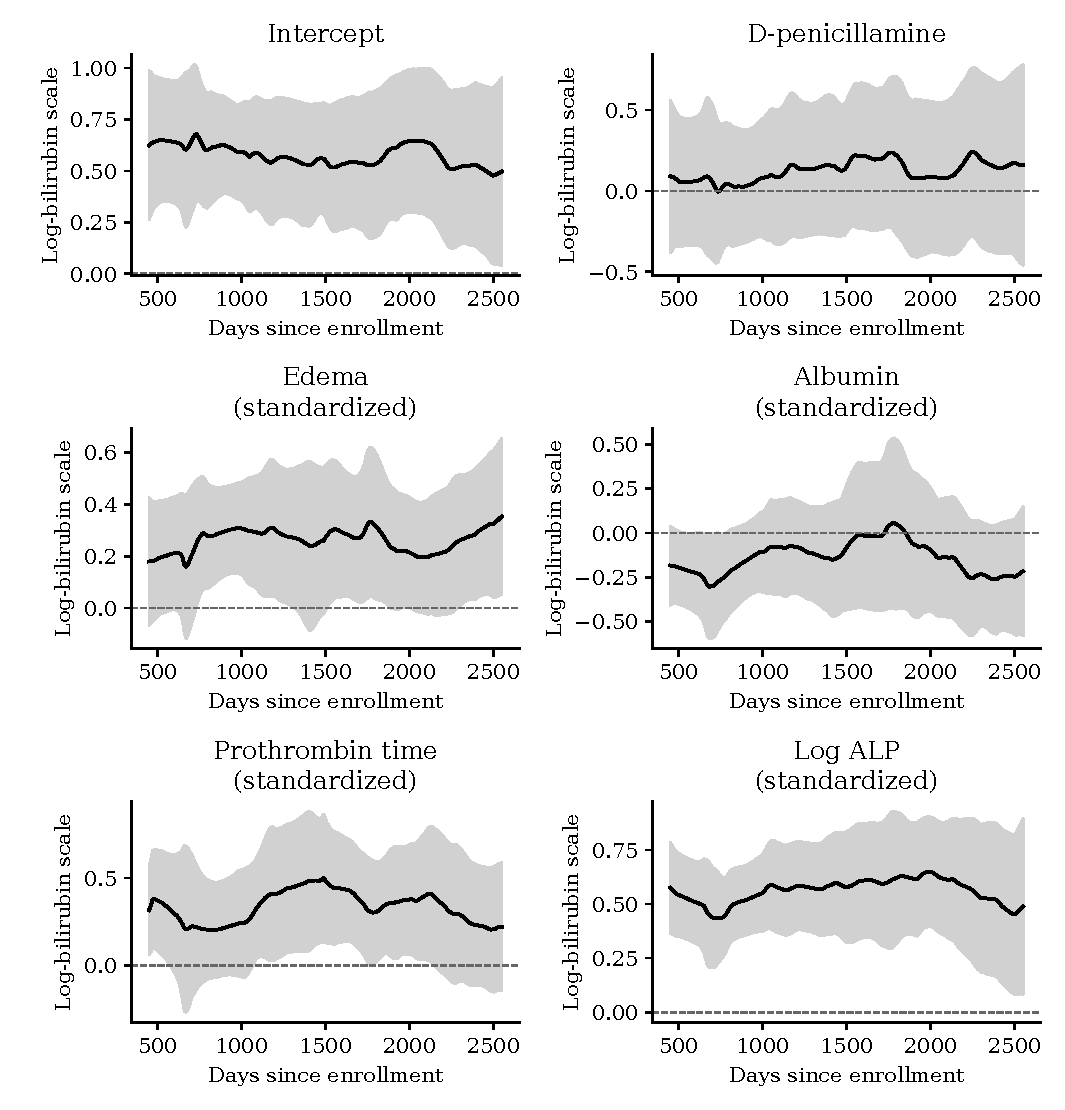
\includegraphics[width=\linewidth]{results/realdata/pbc_vcm_bands.pdf}
\caption{PBC coefficient estimates and nominal joint 95\% bands under the working model. Independent visit times and noninformative follow-up are not established for these data.}
\label{fig:pbc-vcm-new}
\end{figure}

In Figure~\ref{fig:pbc-vcm-new}, the treatment band contains zero throughout the displayed interval, while the log-ALP band remains above zero. Edema and prothrombin time have positive exclusions on portions of follow-up; albumin has short negative exclusions. Bandwidth factors 0.8 and 1.2 and a shorter 2,000-day horizon preserve the treatment and log-ALP descriptions but change the shorter exclusions. Full sensitivity results are in Section~\ref{app:numerics}. These are descriptive adjusted associations: conditioning on contemporaneous biomarkers does not identify a randomized treatment effect, and a band containing zero does not establish equivalence.
\FloatBarrier
